\documentclass[a4paper, 11pt]{article}
\usepackage[utf8]{inputenc}
% page margins
\usepackage[top=2cm, bottom=2cm, left=2.5cm, right=2.5cm]{geometry}
% profile picture
\usepackage{graphicx}
\usepackage{wrapfig}
% fancy page headers and footers
\usepackage{fancyhdr}
% hyperlink support
\usepackage[hidelinks]{hyperref}
% font
\usepackage{paratype}
\usepackage[T1]{fontenc}

\pagestyle{fancy}
\headheight 14pt
\linespread{1.1}

\newcommand{\worktime}[1]{
    \hfill \begin{normalsize}#1\end{normalsize}
}

\begin{document}

% fancy header setup
\lhead{Adrian Göransson - CV}
\chead{}
\rhead{\today}
\lfoot{
    \begin{small}
        \url{http://adriang.se}
    \end{small}
}
\cfoot{}
\rfoot{\thepage}
\renewcommand{\headrulewidth}{0.4pt}
\renewcommand{\footrulewidth}{0.4pt}

% title
    \begin{center}
        \begin{Huge}
            Adrian Göransson
        \end{Huge}

        \begin{large}
            Software developer and network technician
        \end{large}

        +46 709 22 67 19 or \href{mailto:adrian@adriang.se}{adrian@adriang.se}
    \end{center}

% main content
    \section*{Presentation}

        % picture of me!
        \begin{wrapfigure}{r}{0.4\textwidth}\centering
            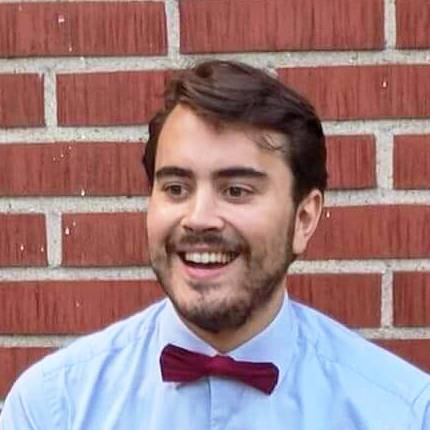
\includegraphics[width=5.5cm]{profile.jpg}
        \end{wrapfigure}

        I'm a 21 year old software developer and network technician based outside Malmö, Sweden.

        My development focuses mainly on the web.
        I have experience with building RESTful APIs in PHP and Python backends.
        I've also built single page apps to communicate with said APIs using popular Javascript and CSS frameworks.

        Programming first started out as a hobby for me when studying network technology at school.
        Today I'm proud to be certified by Cisco with a CCNA.
        Being one of only two students at my school during my time there to receive the certification.
        Knowledge in routing, switching, firewalls and IPSec (VPN).

        I like flying, and my next goal is to take a private pilot's license which I'm currently studying for.

    \section*{Education}

        \subsection*{NTI-Gymnasiet Lund (Cisco Academy)\worktime{2010-2013}}

            IT program with an initial focus on web design and computer internals during the first year.
            Second and third year focus shifted to network and Cisco technologies.
            Graduated with a Cisco CCNA certification.

    \section*{Work experience}

            \subsection*{Beepsend AB \worktime{2013-}}

                Beepsend is an SMS company specializing in ATP (application to peer) messaging.\\
                I've helped build its customer portal as well as internal administrative tools.
                Single page apps built with Chaplin js and Bootstrap using Coffeescript and LESS.

                I've worked with the internal and public APIs that are made in PHP using the Slim framework,
                Redis for caching and MySQL + MySQL Cluster as a database backend.
                RabbitMQ is used for instant messaging and a socket server written in
                Python brings instant updates to the frontend via Websockets.

                Network administrations work has included setting up IPSec VPNs towards clients
                using the software OpenSwan on Linux servers.\\
                I've also set up and maintained Beepsend's SMSC and STP as well as the SS7 and SIGTRAN
                connections that connects to some of the worlds biggest signaling providers
                in order to provide cheap and reliable messaging.

            \subsection*{CDON Group \worktime{2012}}

                I worked at CDON Group for 5 weeks as part of an internship.
                My primary purpose was internal IT support for some 250 people with a
                big focus on Microsoft enterprise deployment solutions.

    \section*{Languages}
        Swedish (native language) and English fluently.

    \section*{Programming experience}

        \subsection*{Web developer}
            \begin{itemize}
                \item HTML5.
                \item CSS3, SCSS (SASS) and LESS.
                \item Javascript and Coffeescript development.
                \item Javscript frameworks: Chaplin, Backbone.js and AngularJS.
                \item CSS frameworks: Bootstrap.
            \end{itemize}

        \subsection*{PHP developer}
            \begin{itemize}
                \item Web development.
                \item API development.
                \item MySQL databases as database backend.
                \item Redis used for caching.
            \end{itemize}

        \subsection*{Python developer}
            \begin{itemize}
                \item Web development with Flask.
                \item Command line scripts.
            \end{itemize}

        \subsection*{Others}
            \begin{itemize}
                \item Experienced user of Git for version control.
                \item Shell scripting in Bash and Zsh.
                \item Some experience with Objective C and iOS development.
                \item Writing in \LaTeX.
            \end{itemize}


    \section*{Systems and networks experience}

        \subsection*{Network}
            \begin{itemize}
                \item Cisco networking equipment and protocols.
                \item Setting up and administrating small to medium sized networks.
                \item IPSec.
                \item Routing protocols.
                \item Switching.
            \end{itemize}

        \subsection*{Systems}
            \begin{itemize}
                \item Linux (Debian and Ubuntu) servers.
                \item Apache, Nginx.
                \item Iptables.
                \item OpenSwan (IPSec).
                \item OpenVPN.
                \item DnsMasq.
            \end{itemize}

        \subsection*{Telephony}
            \begin{itemize}
                \item SS7.
                \item SIGTRAN (M2PA).
                \item SCCP.
                \item Cisco ITP.
            \end{itemize}

    \section*{Miscellaneous}
        \begin{itemize}
            \item Driver's license (Car/class B).
            \item Experienced in Adobe's Creative Suite and especially proficient in Photoshop.
            \item Uses Mac OSX on a daily basis. Very experienced with Windows and Linux desktop environments as well.
        \end{itemize}

% phew, finally
\end{document}
